\documentclass[../main.tex]{subfiles}
\renewcommand{\bm}[1]{\mathbf{#1}}

\begin{document}

\section{Preliminaries}
Note that

\begin{align*}
    np.dot(A,x) = Ax \\
    np.dot(x,A) = x^TA \\
    A @ B = np.matmul(A,B) = AB \\
    np.dot(x,y) = x^Ty \\
\end{align*}


\section{Lecture 1}{Rounding, Approximation, Well Posedness}

\begin{definition}
    We say that a problem is well posed if its solution exists, is unique and depends continuously on the inputs.
\end{definition}

\begin{definition}
    Rounding error refers to our representation of real numbers as floating point numbers.
\end{definition}

\begin{definition}
    Truncation error refers to our representation of infinite collections as finite ones. For example, the truncation of a Taylor
    series to a finite quantity of terms is an example of truncation.
\end{definition}

\begin{definition}
    Approximating a solution can be divided into two stages: approximation before the calculation and approximation during the calculation. Approximation before the calculation includes the following:

    \begin{outline}
        \1 How we model the problem.
        \1 The accuracy of our input data.
        \2 How we measure the input data
        \2 How we compute the input data
    \end{outline}

    Approximation during the calculation includes:

    \begin{outline}
        \1 Rounding Error
        \1 Truncation Error
    \end{outline}

    \begin{remark}
        Recall that norms allow for constant pullout, satisfy the triangle inequality and output $0$ if and only the input to the
        norm is also $0$.
    \end{remark}

\end{definition}

\begin{example}
    It is easy to undestand rounding and truncation error. The first set of approximations can be understood as follows:

    Suppose we use the surface area of the earth as an input. To calculate the surface area, we first assume that the earth
    is a sphere, then we somehow measure the radius and then we compute that area by multiplying the radius squared by $\pi$.
\end{example}
\section{Lecture 2}{Rounding and Error}


\begin{definition}
    Let $x$ be some input, $f$ some true function and $\hat{f}$ some estimated function. Absolute forward error is the difference
    $\abs{f(x) - \hat{f}(x)}$. Relative forward error is $\frac{\abs{f(x) - \hat{f}(x)}}{\abs{f(x)}}$.
\end{definition}

\begin{definition}
    Backward error is the difference between the original input and the input that, under the true function $f$, would have given
    you $\hat{f}(x)$, the output of the original input under the approximate function.
\end{definition}

\begin{center}
    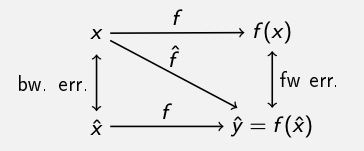
\includegraphics[width=\textwidth,height=\textheight,keepaspectratio]{backward_error}
\end{center}

\begin{remark}
    Suppose I present to you two problems $p_1$ and $p_2$ that have the same forward error but the backward error of $p_1$, $b(p_1)$ is
    such that $b(p_1) > b(p_2)$. Is problem $1$ or $2$ more favorable? Is any more favorable? We can generally say that $p_1$ is more favorable, because it takes a larger input perturbation in $p_1$ to produce, under a true function $f$, the same output perturbation as $p_2$. This would suggest that $p_1$ is more \textit{well conditioned}.
\end{remark}

\begin{remark}
    Truncation and rounding error make up the ways in which an operation is approximate. By truncation error, we refer to the process of replacing infinite sums and expressions with finite ones and by rounding error, we refer to the error introduced in representing real numbers with computer based number systems.
\end{remark}

\begin{lemma}
    This is sort of a lemma:

    The relative error in the forward error tells us how many digits are significant in our estimate of the solution to a problem.
\end{lemma}

\begin{example}
    Suppose we estimate $\sqrt{2} = 1.414\dots$ as $1.4$. Then the negative $\log$ of the relative error is $-\approx \log(0.01) = 2$, meaning
    that (correctly) our estimate is accurate up to $2$ digits.
\end{example}

\begin{definition}
    The condition number is 

    \[
        \sup_{x \in \text{domain}} \frac{\text{Relative Forward Error}}{\text{Relative backward error}}
    \]
\end{definition}

\begin{theorem}
    Assuming that a true function $f$ is differentiable, then its condition number is given by 

    \[
        \sup_{x \in \text{Domain}}\frac{x f'(x)}{f(x)}
    \]
\end{theorem}

\begin{proof}
    \begin{align*}
        \Delta y &= \frac{f(x + \Delta x) - f(x)}{1} = f'(x) \Delta (x) \\
        &\implies \frac{\Delta y}{y} / \frac{\Delta x}{x}  \\
        &= \frac{f'(x) \Delta x}{y} / \frac{\Delta x}{x}  \\
    \end{align*}

    and the latter simplies to the claimed expression.
\end{proof}


\begin{problem}{Forward Error}
    Approximate $f(x) = 1/x$ by the taylor expansion $1 - (x - 1)$. What is the forward error when we let $x = 0.5$?
\end{problem}

It is 0.5

\begin{problem}{Backward Error}
    What about the backward error if we use $x = 0.5$
\end{problem}
We need to find the value $x'$ such that $f(x') = 1.5$. That is $x' = \frac{2}{3}$. Therefore, $\abs{x - x'} = 0.16$.


\begin{problem}{Condition Number}
    Determine the condition number of $\sin(x)$ on the interval $[0 , \pi/2]$.
\end{problem}
\begin{proof}
    The formula gives us that $k(f) = \sup_{x \in [0, \pi/2]} \frac{x \cos x}{\sin x}$. Note that this is a decreasing function on.
    the given interval, so that the largest value is taken on at $x = 0$. By L'Hopital's rule, that gives us:

    \[
        \frac{\cos x - x \sin x}{\cos x}.
    \]

    which evaluates to $1$ at $x = 0$. Thus, the condition number is $1$.
\end{proof}

\begin{problem}{Larger Condition Number}
    Over which interval is the condition number larger: $[0, 2\pi]$ or $[10^4 \pi, 10^4 \pi + 2 \pi]$.
\end{problem}
\begin{proof}
    Recall that the formula is $\frac{x f'(x)}{f(x)}$, and that $f'(x)$ and $f(x)$ will assume the same values up to 
    equivalence classes of $\sin.$ Thus, the $x$ in the numerator accounts for any potential difference, making the second
    interval have a greater condition number.
\end{proof}

\begin{definition}
    A problem is well conditioned if, when considering a problem,
    small perturbations in an input do not result in large perturbations in the problem's output.
\end{definition}

\begin{definition}
    A method is stable if, when using it to solve a problem, the solution produced by the method is an exact solution to a nearby problem (ie the same problem applied to a different input). In other words, the error introduced by the method is no worse than the introduction of a little error into the input data.
\end{definition}


\begin{remark}
    We see that conditioning describes a problem, whereas stability describes a method used to solve that problem.
\end{remark}

\begin{definition}
    A method is accurate if it produces solutions that are very close to the true answer. A solution is accurate if both the method
    is stable and the problem well conditioned. If a problem has a stable algorithm but is not itself well conditioned, then 
    the solution may not necessarily be accurate.
\end{definition}


\section{Lecture 3: Floating Point}

The following questions were prelecture questions:

\begin{problem}{Operator Conditioning}
    Let $x > 1$. Which of $f(x) = 3x, f(x) = 3/x, f(x) = 3-x, f(x) = \sqrt{x}$ is ill posed (here, make the restrictive definition that a well posed problem must have a finite condition number.? 
\end{problem}
\begin{proof}
   We can compute the condition numbers using the formula $xf'(x)/f(x)$ since all functions are differentiable over the domain $x > 1$. This gives:

   \begin{outline}
       \1 \[
           \frac{3x}{3x} = 1
       \]
       \1 
       \[
           \frac{x (-3/x^2)}{3/x} = \frac{(-3/x)}{3/x} = -1
       \]
       \1 \[
           \frac{x (-1)}{3 - x} \to \infty \text{ as } x \to 3
       \]
       \1
       \[
           \frac{-1/2}{\sqrt{x}}
       \]
   \end{outline}
\end{proof}

\begin{problem}{Forward and Backward Errors}
    Approximate $\sqrt{1 + x}$ by $1 + x/2$. What is the absolute
    backward error using $x = 8$.
\end{problem}

\begin{proof}
    To get $1 + 8/2 = 5$ using $f$, we need to let $x = 24$. Hence,
    the absolute backward error is $\abs{8 - 24} = 16$.
\end{proof}

\begin{problem}{Why choose a stable algorithm?}
    A stable algorithm always:
    \begin{outline}
        \1 produces an accurate result
        \2 False. If a problem is additionally well conditioned, then
        a stable algorithm applied to it may result in an accurate solution; otherwise, no
        \1 insensitive to data error
        \2 No, a stable algorithm only assures us that an answer is a solution to a nearby problem
        \1 improves the conditioning of the problem
        \2 No, this is distinct from stability. See the first retort.
        \1 gives the correct answer to a nearby problem
        \2 This is exactly the definition.
    \end{outline}
\end{problem}

\begin{problem}{Condition Number of Square Root}
    At $x = 7$?
\end{problem}
\begin{proof}
    \[
        \frac{1/2}{\sqrt{x}}x \bigg/ \sqrt{x} = 1/2
    \]
\end{proof}

\begin{problem}{Backward Error}
    Given $x = 0.5$, approximate $\cos x$ by $1 - \frac{x^2}{2}$.
    What is the backward error?
\end{problem}

\begin{proof}
    Find $\hat{x}$ such that $\cos \hat{x} = 0.875$. Subtract that
    from $0.5$.
\end{proof}

\begin{problem}{Estimate Condition Number}
    Estimate $f(x) = \log(1 + x)$ (remember that $\log$ means natural
    log) with $x - \frac{x^2}{2} + \frac{x^3}{3}$. Suppose we know that
    $f(0.5168967) = \hat{f}(0.5)$. Then we know that the relative backward
    error is $\frac{0.516897 - 0.5}{0.5}$. Now use this information
    to approximate the condition number of $f$.
\end{problem}

\begin{proof}
    We already know the relative backward error, and the condition number is relative forward error over relative backward error. Hence, the
    condition number estimate is

    \[
        \frac{\hat{f}(0.5) - f(0.5)}{f(0.5)} \bigg/ \text{ Relative Backward Error}
    \]
\end{proof}


\begin{definition}
    Suppose that we represent numbers using 64 bits. 32 bits will be dedicated to the whole portion of any number -- we will progress under this system, going from rightmost bit to left most bit, from $2^0$ to $2^32$; similarly, 32 bits will be dedicated to the fractionalpart of any number -- we will progress from rightmost bit to leftmost bit from $2^-32$ to $2^-1$.
\end{definition}

\begin{remark}
    Suppose that we wish to represent $2^{32}$. Observe that largest number representable using this scheme is $2^{32} - 2^{-32}$.

    It follows that the relative error of our represntation of $2^{32}$ is 

    \[
        \frac{2^{-32}}{2^{32}} = 2^{-64}
    \]

    Now suppose that we wish to represent some number $x$ in the range $(2^{-32}, 2^{-31})$. Assuming that $2^{-32}$ is closer to this
    number then $2^{-32}$, the relative error of this representation is 
    \[
        \frac{\abs{x - 2^{-32}}}{\abs{x}} \leq \frac{\abs{2^{-33}}}{\abs{x}} \leq \frac{\abs{2^{-33}}}{2^{-32}} = 2^{-1}
    \]

    Observe that whereas the relative error in the former is good, in the latter it is poor. This motivates our definition of the
    double precision floating point system.
\end{remark}

\begin{example}
    Represent $13$ in scientific notation in a binary number system. Require that the first and only digit before the decimal point (remember that this is scientific notation) is a $1$; further require that $1$ must occupy this position.  You will find that the representation is uniquely $(1.101)_2 * 2^3$.
\end{example}

\begin{remark}
    Suppose I told you that we we will represent all numbers as we did above. Leaving aside how we would represent $0$, observe that since we require that the first and only digit before the decimal point is a $1$, if we want to store such representations, there is no point in storing the $1$. This allows us to say the following:
\end{remark}

\begin{definition}

    \begin{outline}
        \1 The double precision floating point system allocates $52$ bits to store the fractional part of a number represented using the scheme above, where a $1$ in the units place implicitly precedes the fractional part.
        \1 $11$ bits are allocated to store an exponent and $1$ bit is allocated to store a sign bit.
        \2 The $11$ exponent bits allow us to get integers in the range $[0,2047]$. Assuming that we begin with an offest of $-1023$,
        meaning that $0$ maps to $-1023$, we can represent an exponent in the range $[-1023, 1024]$.
        \1 When the exponent becomes $0$, instead of mapping to $-1023$, we to $-1022$ (yes, this contradicts the previous line, but
        introducting the contradiction and then correcting it is pedagogically more gradual). We also do away with the implicit $1$ that precedes
        the fractional part of the significand (recall tha the fractional part of the significand is the only part which is stored in our representation). $0$ is represented if we let all bits of the fractional part be $0$.
        \2 Since we are no longer required to have an implicit, leading $1$, notice that we can now drop down past $1 * 2^{-1022}$. Represent
        $2^{-1023}$ as $0.100\dots \times 2^{-1022}$; represent $2^{-1024}$ as $0.0100\dots \times 2^{-1022}$ and so forth. UNRESOLVED
        \1 We map $2^{1024}$ to $\infty$ and if the fractional part contains any non-zero digit, we call that values $\infty$ instead. UNRESOLVED
        \1 Define the UFL and OFL to be the smallest and greatest normal numbers that are not subnormal nor $\infty$.
    \end{outline}
\end{definition}

\begin{definition}
    Suppose that we have a number $x = b.\underbrace{b_1b_2\dots b_{52}}_{\text{all useable digits consumed}}d_1d_2d_3$. We need to somehow represent
    $x$ in our floating point system. To do so, we round on the basis of $d_1d_2d_3$. Now we could make the scheme round to nearest, meaning that
    add $1$ to $b_{52}$ if $d_1d_2d_3 > 100$ and do nothing if $d_1d_2d_3 < 100$, but we must then choose what to do when $d_1d_2d_3 = 100$. What
    then? If we make the consistent, arbitrary decision to round up, we will produce statistical noise. Thus, the scheme employed is to round to even: \\

    If $b_{52}$ is 0, then do nothing, so that $x$ is even; if $b_{52}$ is $1$, then add $1$ to $b_{52}$.
\end{definition}



\begin{remark}
    Some floating point exercises \url{https://relate.cs.illinois.edu/course/cs450-s19/flow/inclass-floating-point/start/}
\end{remark}

\begin{definition}
    Let $\e$ be the smallest number such that $\text{fl}(x(1 + \e)) > x$. If we use round to even, it is $2^{-52}$; if we use round to nearest,
    with rounding up in case of a tie, it is $2^{-53}$ -- in which case we also distinguish $2^{-52}$ with some title.
\end{definition}

\begin{lemma}
    The relative error in representing any number $x$ within the normal range is at most $\e$.
\end{lemma}

\begin{proof}
    Given $x$, there is an $a$ such that

    \[
        2^{a} \leq x \leq 2^{a+1}
    \]

    Since we can represent any number $y = 2^{a} + \e * n$ up
    to $y = 2^{a+1}$, it follows that there is at least one representable number in the range $[x, x + \e]$. This allows us to say that the absolute error between this number and $x$ is at most $\e$, which is formalized below:


    \[
        \frac{\abs{x - (1 + \e)x}}{\abs{x}} = \frac{\abs{x} \e}{\abs{x}} = \e
    \]
\end{proof}

\section{Lecture 4}

\subsection{Quiz}
\pp{1}
Estimating Output Error with Condition Numbers
A function f(x) has a condition number of $2.3×10^2$. For x=65 with an absolute error Δx=5×10−5, what is an upper bound on the relative error of the output?

TIP: On any quiz/exam question where you are asked to enter a number, you can also enter an expression, which will be evaluated for you. No need to bring out the calculator. (I.e. in the box below, you could simply enter "100*13", which would count the same as entering "1300".)

Make sure your answer has at least two accurate digits.

\begin{solution}
    Relative Error <= Relative Input Error * Condition Number
    Relative Error <= (Machine Epsilon or some problem specific relative input error) * condition Number
    <= $(5 * 10^-5)/(65) * 2.3 * 10^2$
\end{solution}

\pp{2}

Floating Point Rounding
What is the value of 2‾√×π when calculated in a decimal floating point system with 3 digits that uses rounding? (Apply rounding to both the input data and the result of the arithmetic.)

\begin{solution}
    $\sqrt{2} \approx 1.41$ and $\pi \approx 3.14$. Multiply both and round to $3$ decimal places.
\end{solution}

\pp{3}
In a normalized floating point system that supports subnormal numbers, which of the following binary operations on two positive numbers could lead to overflow?

\begin{solution}
    Addition, Multiplication and Division can all lead numbers to explode outside of the normalized floating number range.

    If two addends are already normalized floating point numbers, however, then there is no chance that subtracting these numbers can lead to a result that is not a normalized floating point\footnote{Recall that a normalized floating point number has $1$ in the fractional part before the significand.}
\end{solution}

\pp{4}
1 point
Machine Epsilon and UFL
Which of the following statements are true?

Select all that apply:
Machine epsilon places a lower bound on the magnitude of normal floating point numbers.
Machine epsilon is determined by the number of bits in the significand.
Machine epsilon places an upper bound on the relative error of representing a real number in a floating point format.
The UFL is determined by the number of bits in the exponent.

\begin{solution}
    The bottom $3$ are correct; the first is wrong, because the magnitude of normal floating point numbers is determined by the exponent range; the second is correct, because machine epsilon is $\beta^{-(p-1)}$ where $\beta$ is a base and $p$ a precision; the third is correct, because given a floating point number $y$, the smallest perturbation to $y$ that results in a different floating point number is $\e \abs{y}$. The fourth is correct, because the order of magnitude of UFL is $\beta^{L+1}$ where the exponent range falls in $\left[ L,U \right]$.
\end{solution}

\pp{5}
Floating Point Relative Error
Which of the following is closest to the relative error from representing $e×2−145$ in IEEE single precision.

\begin{solution}
    Notice that $e \times 2^{-145}$ is subnormal number. The underflow limit for single precision IEEE floating point numbers is $2^{-126}$. Anything smaller requires that the leading $1$ be shifted along the fractional part of a number. Since $e \times 2^{-145} \approx 2^{-144}$, it follows that we need to shift the leading $1$ $18$ units to the right of the decimal. This will leave $5$ digits (bits) in the fractional component for futher reprsentation. If we have $n$ digits, then our relative error is approximately $\beta^{-n}$. Whence, the relative error here is $2^{-5}$.
\end{solution}

\pp{6}
Properties of Floating Point Operations
Which of the following is true for floating point multiplication and addition?
Select all that apply:
Floating point addition is associative.
Floating point multiplication is commutative.
Floating point multiplication is associative.
Floating point addition is commutative.
\begin{solution}
    Floating point multiplication and addition are commutative but not associative.
\end{solution}

I skip problem 7 -- if you understood the solution to an earlier problem, you'll be okay.

\begin{example}
    To perform floating point addition, suppose that you have
    $b_0.b_1 \dots b_n \times 2^{x}$ and 
    $d_0.d_1 \dots d_n \times 2^{y}$ where $x > y$; make sure
    that you multiply the second number by $2^{x-y}$ and then perform grade school addition.
\end{example}

\begin{definition}
    Catastrophic cancellation takes place when the number of
    accurate digits in the result of an operation are far
    less than the number of accurate digits in the members
    of that operation.
\end{definition}

\begin{example}
    Supposing that we opereate in double precision and that
    $a$ and $b$ both have 12 digits of accuracy. Suppose
    that $a$ and $b$ agree up to their first 10 digits.

    When $a$ and $b$ are subtracted, the first $10$ digits
    will be cancelled and the final 2 digits will shift
    leftwards, becoming the $2$, sole accurate digits. The
    remaining digits will be filled with garbage. From this,
    we see that whereas we had 12 digits of accuracy, we now
    only have 2 (ie our relative error is $10^-2$).
\end{example}

\begin{definition}
    Given a vector norm $\norm{\cdot}$, we define the matrix norm to be

    \[
        \sup_{x \in \mc{D}, x \not = 0} \frac{\norm{Ax}}{\norm{x}}
    \]

    This is equivalent to

    \begin{align*}
        \sup_{x \in \mc{D}, x \not = 0} \frac{\norm{Ax}}{\norm{x}} \\
        \sup_{x \in \mc{D}, x \not = 0} \frac{\norm{A\frac{x}{\norm{x}}}}{1} \\
        \sup_{x \in \mc{D}, \norm{x} = 1} \frac{\norm{Ax}}{1} \\
    \end{align*}

    We denote this norm by $\norm{A}$.
\end{definition}

\begin{proposition}
    \[
        \norm{A} \norm{x} \geq \norm{Ax}
    \]

    for all $x$ that $A$ can multiply.
\end{proposition}

\begin{proof}
   Follows by definition. 
\end{proof}

\begin{proposition}
   \[
       \norm{A}_1 = \max_{j} \sum_{i}^{}\abs{A_{i,j}}
   \]

   \[
       \norm{A}_{\infty} = \max_{i} \sum_{j}^{}\abs{A_{i,j}}
   \]

   An easy way to remember the $1$ norm and $\infty$ norm is to note that these matrix norms also
   coincide for a vector, for which the $1$ norm is the sum of absolute values, and the $\infty$ norm is the maximum value.
\end{proposition}

\begin{definition}
    Suppose that $A$ is invertible and that we wish to find the condition number of the problem of solving $Ax = b$ where
    $b$ is the input and $x$ the ouput; then the condition number is given by 

    \[
        \frac{\norm{\Delta x}}{\norm{x}} \bigg/ \frac{\norm{\Delta b}}{\norm{b}}
    \]

    \begin{align*}
        & \frac{\norm{\Delta x}}{\norm{x}} \bigg/ \frac{\norm{\Delta b}}{\norm{b}} \\
         \intertext{Let $x = \inv{A}b$ and $\Delta x = \inv{A}\Delta b$} \\
        & \frac{\norm{\inv{A}\Delta b}}{\norm{\inv{A}b}} \bigg/ \frac{\norm{\Delta b}}{\norm{b}} \\
         \intertext{Now apply submultiplicativity} \\
         & \leq \norm{A} \norm{\inv{A}} \\
         \intertext{This inequality can be shown to be sharp for every matrix: for every matrix, there is a vector $b$ 
             for which this bound is attained, and so the condition number of the problem is $\norm{A}\norm{\inv{A}}$} \\
    \end{align*}

    We also call this quantity the condition number of the matrix.
\end{definition}

\begin{definition}
    If a matrix is not invertible, then we say that $k(A) = \infty$.
\end{definition}

\begin{proposition}
    $k(A) = k(\inv{A})$ and matrix vector multiplication has the same conditioning as solving a system of linear equations.
\end{proposition}

\begin{proof}
    The first is easy. To find the $y$ such that $Ax = y$, take $x$ as the input of $\inv{A}y = x$.
\end{proof}

\begin{proposition}
    \begin{outline}
        \1 The following properties hold:
        \2 $\norm{AB} \leq \norm{A} \norm{B}$
        \3 For $\norm{ABx} \leq \norm{A}\norm{Bx} \leq \norm{A} \norm{B} \norm{x}$. The previous was true for all $x$; in particular,
        for all $x \not = 0$, this implies that

        \[
            \norm{AB} = \frac{\norm{ABx}}{\norm{x}} \leq \norm{A}\norm{B}
        \]
        \2 $\norm{A + B} \leq \norm{A} + \norm{B}$.
        \2 $\norm{A \inv{A}} = 1 \leq \norm{A} \norm{\inv{A}} \implies 1 \leq k(A)$
        \1 $k(\gamma A) =  k(A)$.
        \1 $\norm{\gamma A} =  \gamma \norm{A}$.
        \1 $k(A) = \max_{x \not = 0} \frac{\norm{Ax}}{\norm{x}} (\min_{x \not = 0}\frac{\norm{Ax}}{\norm{x}})^{-1}$
        \2 
        \begin{align*}
            \intertext{By definition:} \\
            \norm{\inv{A}} = \max_{x \not = 0}\frac{\norm{\inv{A}x}}{\norm{x}} \\
            \intertext{Let $y = \inv{A}x$, meaning that $Ay = x$. Then} \\
            = \max_{x \not = 0}\frac{\norm{y}}{\norm{Ay}} \\
            \intertext{Since $y = \inv{A}y$, we can consider the $\max$ over $y$ instead of $x$:} \\
            = \max_{y \not = 0}\frac{\norm{y}}{\norm{Ay}} \\
            = \inv{(\min_{y \not = 0}\frac{\norm{Ay}}{\norm{y}})} \\
        \end{align*}
        \1 If $D$ is a diagonal matrix, then $k(D) = \frac{\max{d_{i,i}}}{\min_{d_{i,i}}}$
        \1 An orthogonal matrix has norm $1$ in any norm.
    \end{outline}
\end{proposition}

\begin{remark}
    A computational technique to evaluating a condition number is multiply a matrix $A$ by many vectors that have unit norm and take
    the maximum norm of the resultant vectors divided by the minimum norm of the resultant vectors.
\end{remark}











\end{document}
